\newpage
\section{Support Vector Machine (SVM)}

\subsection{Lineare Trennbarkeit von Daten}
\subsubsection{Allgemeines}

\myul{\textbf{Datenpunkte:}} (2D Beispiel)\\
\begin{tabular}{lllll}
    $A:(\underbrace{(x_1,x_2)}_{\vec{x}_1};y_1)$, &
    $B:(\underbrace{(x_1,x_2)}_{\vec{x}_2};y_2)$, &
    $C:(\underbrace{(x_1,x_2)}_{\vec{x}_3};y_3)$, & 
    $\cdots $, &
    $N:(\underbrace{(x_1,x_2)}_{\vec{x}_n};y_n)$\\
\end{tabular}

$\vec{x}_j$ sind Datenvektoren\\
$y_j$ $\in $ \{$\pm 1$\} klassifiziert die jeweiligen Datenvektoren
\newline
\begin{minipage}[]{0.56\columnwidth}
    \myul{\textbf{Hyperebenen:}}\\
    $\boxed{\vec{w}^{tr}\cdot\vec{x}+b=0}$ \\
    $\vec{w}$: Normalenvektor, $\vec{w} \in \mathbb{R}^d$ und $\vec{w} \neq 0$\\
    $b$: Konstante, $b \in \mathbb{R}$\\
    Dimmension der Hyperebene $= d-1$\\
    Abstand der Hyperebene zum Ursprung: $\frac{\left\lvert b \right\rvert }{\left\lvert \vec{w}\right\rvert }$
    \medskip

    \myul{\textbf{Klassifizierung:}}\\
    $\boxed{\vec{w}^{tr}\cdot\vec{x}+b>0} \Rightarrow \vec{x} $ gehört zur Klasse $y = +1$\\
    $\boxed{\vec{w}^{tr}\cdot\vec{x}+b<0} \Rightarrow \vec{x} $ gehört zur Klasse $y = -1$
    \medskip

    \myul{\textbf{Klassifizierung der Trainigsdaten:}}\\
    $\boxed{\vec{w}^{tr}\cdot\vec{x}_j+b \geq 0} \Rightarrow \vec{x}_j $ gehört zur Klasse $y = +1$\\
    $\boxed{\vec{w}^{tr}\cdot\vec{x}_j+b\leq 0} \Rightarrow \vec{x}_j $ gehört zur Klasse $y = -1$
    \medskip

    \myul{\textbf{Zielfunktion:}}\\
    $\boxed{\frac{2}{\left\lvert \vec{w}\right\rvert }=\frac{2}{w}}$
\end{minipage}\hfill
\begin{minipage}[t]{0.4\columnwidth}
    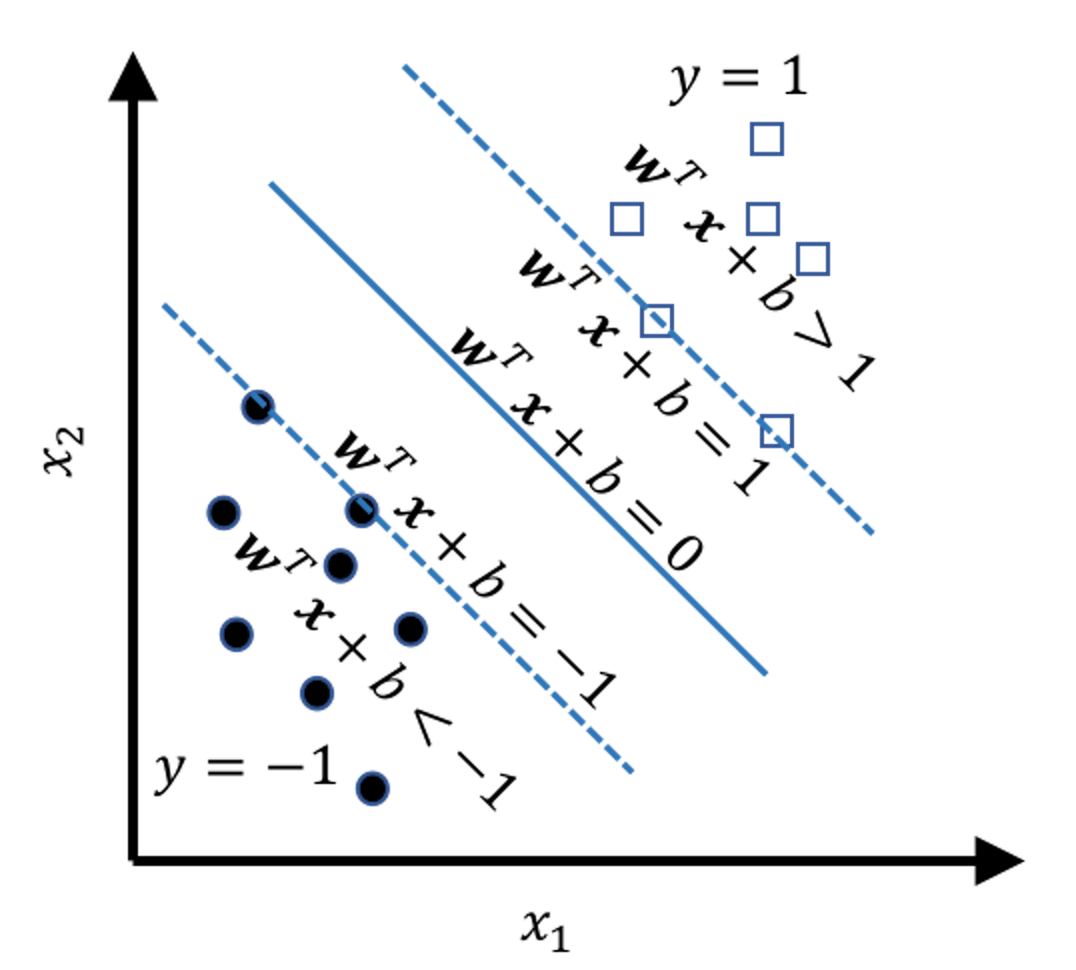
\includegraphics[width=4cm]{images/7_model_values.png}
\end{minipage}

\subsubsection{Das primale Optimierungsproblem}
$\boxed{\frac12\vec{w}^{tr}\cdot\vec{w}=\frac12\left|\vec{w}\right|^2=\frac12w^2\to\min!\quad\mathrm{s.t.}\quad\left(\vec{w}^{tr}\cdot\vec{x}_j+b\right)y_j\geq1\quad\left(j=1,\cdots,N\right)}$

\subsubsection{Das duale Optimierungsproblem}
\myul{\textbf{Nebenbedingung:}}\\
$\boxed{\underbrace{1-\left(\vec{w}^{tr}\cdot\vec{x}_j+b\right)y}_{g_j(\vec{w}^{tr},b)}\leq0\Leftrightarrow g_j(\vec{w}^{tr},b)\leq0\quad\left(j=1,\cdots,N\right)}$
\medskip

\myul{\textbf{Lagrange-Funktion:}}\\
Zusammengesetzt aus dem primalen Problem und den Nebenbedingungen.\\
\begin{tabular}{|r@{ }l|}
    \hline
    $L(\vec{w}^{tr},b,\vec{a})$ & $ =L(w_1,w_2, ...,w_d,b,\alpha_1,\alpha_2, ...,\alpha_N) $ \\
                                & $ =\frac12\vec{w}^{tr}\cdot\vec{w}+\sum_{j=1}^N\alpha_j\left(\underbrace{1-\left(\vec{w}^{tr}\cdot\vec{x}_j+b\right)y_j}_{g_j\left(\vec{w}^{tr},b\right)}\right) $ \\
    \hline
\end{tabular}
\medskip

\myul{\textbf{Stationaritätsbedingungen:}}\\
Aus der Bedingung, dass $\grad(L) = 0$ sein muss, lassen sich folgende Formeln ableiten:
$\boxed{grad_{\left\{\vec{w}^{tr},b\right\}}\left(L(\vec{w}^{tr},b,\vec{\alpha})\right)=\vec{0}} \Leftrightarrow 
\boxed{\vec{w}=\sum_{j=1}^N\alpha_jy_j\vec{x}_j} \text{ und }
\boxed{\sum_{j=1}^N\alpha_jy_j=0}$\\
%\myul{\textbf{Lagrange-Funktion mit den Dualvariablen $\alpha_j$:}}\\
%$\boxed{L(\vec{w}^{tr},b,\vec{\alpha})=\sum_{j=1}^N\alpha_j-\underbrace{\frac12\sum_{j,j'=1}^N\alpha_j\alpha_j,y_jy_j,\vec{x}_j^{tr}\cdot\vec{x}_j}_{\frac{1}{2}\vec{w}^{tr}\cdot\vec{w}}:=L(\vec{\alpha})\quad , \alpha_j\geq0}$
\myul{\textbf{Das duale Problem:}}\\
Die oben erhaltenen Summen können nun in die Lagrange-Fkt. eingesetzt werden. Daraus entsteht\\
$\boxed{L(\vec{\alpha})=\sum_{j=1}^N\alpha_j-\underbrace{\frac12\sum_{j,j'=1}^N\alpha_j\alpha_{j'} \space y_jy_{j'} \space \vec{x}_j^{tr}\cdot\vec{x}_{j'}}_{=\frac12 \vec{w}^{tr} \cdot \vec{w}}\quad\to\quad\max!\quad\mathrm{s.t.}\quad\alpha_j\geq0\wedge\sum_{j=1}^N\alpha_jy_j=0}$

\newcolumn
\myul{\textbf{Formulieren des dualen Optimierungsproblems mit den Lagrange-Variablen $\alpha_j$:}}\\
Vorgenehsbeispiel für 3 Datenpunkte:
\begin{enumerate}
    \item \myul{\textbf{Lagrange-Funktion $L(\vec{\alpha}) $ aufstellen:}}\\
    $\boxed{L(\vec{\alpha})=\sum_{j=1}^N\alpha_j-\frac{1}{2}\sum_{j,j'=1}^N\alpha_j\alpha_{j'} \space y_jy_{j'} \space \vec{x}_j^{tr}\cdot\vec{x}_{j'}\quad\to\quad\max!}$\\
\end{enumerate}

\myul{\textbf{Finden der Lagrange-Variablen $\alpha_j$:}}
\begin{enumerate}
    \item \myul{\textbf{Stationaritätsbedingungen aufstellen:}}\\
    \textbf{a: }$\boxed{\alpha_j\geq0} \text{ und } \textbf{b: } \boxed{\sum_{j=1}^N\alpha_jy_j=0} $
    \item \myul{\textbf{Nebenrechnung:}}\\
    \textbf{b} umstellen nach einer Variablen (z.B. $\alpha_1$) und in Lagrange-Funktion ersetzen
    \item \myul{\textbf{Gradient von verkürzter Lagrange-Funktion berechnen und restliche $\alpha$ finden:}}\\
    $\nabla(L_{neu}(\alpha_2 , \alpha_3)) \quad \Rightarrow \alpha_2 = ..., \text{  } \alpha_3 = ...$
    \item \myul{\textbf{Fehlendes $\alpha$ berechnen:}}\\
    $\alpha_2$ und $\alpha_3$ in \textbf{2. b} einsetzen und $\alpha_1$ berechnen
\end{enumerate}

\myul{\textbf{Lösen des dualen Optimierungsproblems:}}
\begin{enumerate}
    \item \myul{\textbf{Normalenvektor $\vec{w}$ finden:}}\\
    $\boxed{\vec{w}=\sum_{j=1}^N\alpha_jy_j\vec{x}_j}$
    \item \myul{\textbf{Konstante $b$ finden:}}\\
    Mit Stützvektor-Datenpunkt aus Klasse $y = +1$:\\
    $\boxed{b = +1 -\vec{w}^{tr}\cdot\vec{x}_{...} = ...}$\\
    Mit Stützvektor-Datenpunkt aus Klasse $y = -1$:\\
    $\boxed{b = -1 -\vec{w}^{tr}\cdot\vec{x}_{...} = ...}$\\
\end{enumerate}









